% ---------------------------------------------------------------------------
% AgentPathTriage
%
% Two column ACM format. To switch to the single column layout that ACM
% journals such as TOPS use for submission, replace sigconf with acmsmall
% below and nothing else changes:
%
%   \documentclass[acmsmall,nonacm,screen]{acmart}
%
% nonacm removes the conference footer and the copyright block, which is what
% an arXiv preprint and a course submission want. Remove it when submitting
% to ACM so the class puts the rights block back.
% ---------------------------------------------------------------------------
\documentclass[sigconf,nonacm,screen]{acmart}

\settopmatter{printacmref=false}
\renewcommand\footnotetextcopyrightpermission[1]{}

% ---------------------------------------------------------------------------
% preamble.tex: packages and macros shared by the whole paper.
% ---------------------------------------------------------------------------

\usepackage{xspace}
\usepackage{booktabs}
\usepackage{multirow}
\usepackage{amsmath}
\usepackage{amssymb}
\usepackage{tikz}
\usepackage{pgfplots}
\pgfplotsset{compat=1.18}
\usetikzlibrary{arrows.meta, positioning, calc}

% --- drafting aids ----------------------------------------------------------
% \todo marks work still to do. \nodata marks a place where the paper
% deliberately reports that something was not measured, which is a statement
% and not a gap. Set \draftmode to 0 before submitting: \todo then raises an
% error so no marker can survive into the final file, and \nodata stays.
\newcommand{\draftmode}{0}

\definecolor{todored}{RGB}{176,0,32}
\newcommand{\todo}[1]{%
  \ifnum\draftmode=1%
    \textcolor{todored}{\textbf{[TODO: #1]}}%
  \else%
    \GenericError{}{Unresolved TODO: #1}{}{}%
  \fi}
\newcommand{\nodata}{\textsl{not measured}\xspace}

\usepackage{algorithm}
\usepackage{algpseudocode}
\usepackage{listings}

% Terraform excerpts: no colour, no bold keywords, just a readable monospace
% block that fits a two column measure.
\lstdefinestyle{tf}{
  basicstyle=\scriptsize\ttfamily,
  commentstyle=\color{cNeutral}\itshape,
  numbers=none, frame=none, showstringspaces=false,
  columns=fullflexible, keepspaces=true,
  breaklines=true, breakatwhitespace=false,
  aboveskip=2pt, belowskip=2pt, xleftmargin=2pt,
  morecomment=[l]{\#}, morestring=[b]",
  escapeinside={(*}{*)}
}
\lstset{style=tf}

% --- naming -----------------------------------------------------------------
\newcommand{\tool}{AgentPathTriage\xspace}
\newcommand{\agentcore}{Amazon Bedrock AgentCore\xspace}
\newcommand{\foundry}{Microsoft Foundry\xspace}

% --- the escalation predicate ----------------------------------------------
\newcommand{\eff}{\ensuremath{\mathrm{eff}}}
\newcommand{\auth}{\ensuremath{\mathrm{auth}}}
\newcommand{\Esc}{\ensuremath{\mathrm{Esc}}}

% --- code and identifiers ---------------------------------------------------
% Two column measure is narrow and an ARN or an API name does not hyphenate,
% so these are declared through the url package, which breaks at the
% punctuation inside them and keeps a typewriter face.
% \allowbreak after the punctuation inside an identifier, so a long ARN can
% break across a narrow column. Robust, because these appear in section titles
% and captions, which are moving arguments.
\DeclareRobustCommand{\bk}[1]{#1\allowbreak}
\DeclareRobustCommand{\api}[1]{\texttt{#1}}
\DeclareRobustCommand{\iam}[1]{\texttt{#1}}

% A little give, so a long identifier stretches a line instead of running into
% the gutter.
\emergencystretch=2em

% Let a page carry more float and less forced text, so a figure does not push
% a nearly empty page to the end of the paper.
\renewcommand{\topfraction}{0.92}
\renewcommand{\bottomfraction}{0.8}
\renewcommand{\textfraction}{0.1}
\renewcommand{\floatpagefraction}{0.75}
\renewcommand{\dbltopfraction}{0.92}
\renewcommand{\dblfloatpagefraction}{0.75}
\setcounter{topnumber}{2}
\setcounter{dbltopnumber}{2}
\setcounter{totalnumber}{4}

% --- figure colours, one place ----------------------------------------------
\definecolor{cIdentity}{RGB}{31,110,160}
\definecolor{cStored}{RGB}{191,84,47}
\definecolor{cNeutral}{RGB}{120,124,131}
\definecolor{cAccent}{RGB}{28,124,84}
\definecolor{cFaint}{RGB}{226,228,232}

% ---------------------------------------------------------------------------
% numbers.tex
%
% Every figure that appears in the paper is defined here once, and every
% definition names the artifact it was read from. Nothing in the body of the
% paper should contain a bare number that is not defined in this file.
%
% The point of the indirection: when an artifact is regenerated, the number
% changes in one place and the paper stays consistent with the evidence. A
% number with no artifact behind it is not defined here, and the text says
% that it is not measured rather than carrying an estimate.
%
% Regenerate the artifacts with: python3 evaluation/reproduce.py
% ---------------------------------------------------------------------------

% --- AWS corpus and analysis population ------------------------------------
% source: evaluation/benchmark/corpus_takeover_census.json
\newcommand{\nProjects}{220\xspace}              % configurations_measured
\newcommand{\nProjectsFailed}{0\xspace}          % configurations_failed

% source: evaluation/benchmark/perf_tier2.json
\newcommand{\nTerraformFiles}{3519\xspace}
\newcommand{\corpusSeconds}{182.1\xspace}
\newcommand{\medianSeconds}{0.888\xspace}
\newcommand{\pNinetySeconds}{1.093\xspace}
\newcommand{\pNinetyNineSeconds}{1.789\xspace}
\newcommand{\maxSeconds}{9.001\xspace}
\newcommand{\peakMemoryMB}{114.6\xspace}

% --- escalation results -----------------------------------------------------
% source: evaluation/benchmark/corpus_takeover_census.json, key "expanded"
\newcommand{\nEscalating}{3\xspace}              % with_an_escalation
\newcommand{\nEscalatingOwnResource}{2\xspace}   % gaining a resource the config writes
\newcommand{\nSurvivingTakeover}{1\xspace}       % with_a_surviving_takeover_edge
\newcommand{\nBlocked}{26\xspace}                % blocked_takeover_candidates
\newcommand{\nBlockedConfigs}{16\xspace}         % configs_with_a_blocked_candidate
\newcommand{\nPassRoleWide}{1\xspace}            % passrole wide enough to cover a sibling

% source: evaluation/benchmark/blocked_takeover_source_check.json
\newcommand{\nBlockedAgentToAgent}{10\xspace}
\newcommand{\nBlockedSingleAgent}{10\xspace}
\newcommand{\nBlockedPrincipalNotAgent}{4\xspace}
\newcommand{\nBlockedTargetNotAgent}{2\xspace}

% --- role sharing -----------------------------------------------------------
% source: evaluation/benchmark/shared_role_corrected.json
\newcommand{\nMultiAgentBlocks}{18\xspace}
\newcommand{\nMultiAgentRuntimes}{20\xspace}
\newcommand{\nSharedRoleBlocks}{5\xspace}
\newcommand{\nSharedRoleRuntimes}{7\xspace}

% --- chain analysis ---------------------------------------------------------
% source: evaluation/benchmark/chain_cfn_corpus.json, key "population"
\newcommand{\nChainTerraform}{18\xspace}
\newcommand{\nChainCfn}{9\xspace}
\newcommand{\nChainDenominator}{27\xspace}
\newcommand{\nChainNotCovered}{44\xspace}
\newcommand{\nChainsFound}{0\xspace}
\newcommand{\chainBound}{10.5\xspace}             % 95 percent upper bound, percent

% source: evaluation/benchmark/chain_cfn_corpus.json, key "cloudformation"
\newcommand{\nCfnMultiRuntime}{12\xspace}
\newcommand{\nCfnAnalysed}{9\xspace}
\newcommand{\nCfnUndecidable}{3\xspace}

% --- CDK synthesis ----------------------------------------------------------
% source: evaluation/benchmark/cdk_synth_chain.json
\newcommand{\nCdkInScope}{38\xspace}
\newcommand{\nCdkAnalysed}{12\xspace}
\newcommand{\nCdkRuntimes}{30\xspace}
\newcommand{\nCdkEscalating}{0\xspace}
\newcommand{\nCdkFailLanguage}{5\xspace}
\newcommand{\nCdkFailLocate}{2\xspace}
\newcommand{\nCdkFailSynth}{17\xspace}
\newcommand{\nCdkFailInstall}{2\xspace}
% source: evaluation/benchmark/chain_cfn_corpus.json, key "cdk"
\newcommand{\nCdkMultiRuntimeDirs}{41\xspace}

% --- Azure AI Foundry survey ------------------------------------------------
% source: evaluation/benchmark/foundry_recon.json
\newcommand{\nFoundryRepos}{360\xspace}
\newcommand{\nFoundryFiles}{45992\xspace}
\newcommand{\nFoundryDirs}{16450\xspace}
\newcommand{\nFoundryAuthValues}{516\xspace}
\newcommand{\nFoundryAuthDirs}{210\xspace}
\newcommand{\nFoundryAgentDirs}{0\xspace}        % dirs holding an agent declaration
\newcommand{\nDisclosureReports}{3\xspace}    % validation/sends, one per channel group
\newcommand{\nDisclosureRepos}{7\xspace}      % repositories covered by those reports
\newcommand{\nDisclosureIssues}{2\xspace}     % sent as a public GitHub issue
\newcommand{\nDisclosureEmails}{1\xspace}     % sent to a vendor security address
\newcommand{\nFoundryTemplateCopies}{11\xspace}  % foundry_template_dup identical_copies
\newcommand{\nFoundryTemplateRepos}{10\xspace}   % repositories_carrying_the_copy
\newcommand{\nFoundryTemplateApiKey}{3\xspace}   % call sites with authType ApiKey
\newcommand{\nFoundryTemplateShared}{7\xspace}   % call sites setting isSharedToAll true
\newcommand{\nFoundryAgentAuthValues}{0\xspace}  % assigned authType values that are agent scoped

% authType values, in the directories that declare a connection resource
\newcommand{\nAuthAAD}{279\xspace}
\newcommand{\nAuthApiKey}{161\xspace}
\newcommand{\nAuthManagedIdentity}{44\xspace}
\newcommand{\nAuthCustomKeys}{13\xspace}
\newcommand{\nAuthProjectManagedIdentity}{8\xspace}
\newcommand{\nAuthAccessKey}{4\xspace}
\newcommand{\nAuthSingletons}{7\xspace}          % one each, see table
\newcommand{\nAuthStoredCredential}{183\xspace}  % ApiKey+CustomKeys+AccessKey+singletons
\newcommand{\nAuthIdentity}{333\xspace}
\newcommand{\pctAuthStoredCredential}{35\xspace} % percent, 183/516

% occurrence counts of markers across the whole Foundry corpus
% source: evaluation/benchmark/foundry_recon.json, key "markers"
\newcommand{\nMarkerAuthType}{1315\xspace}
\newcommand{\nMarkerProjects}{1137\xspace}
\newcommand{\nMarkerMlsConnections}{366\xspace}
\newcommand{\nMarkerFoundryResource}{109\xspace}
\newcommand{\nMarkerProjectManagedIdentity}{60\xspace}
\newcommand{\nMarkerUserEntraToken}{28\xspace}
\newcommand{\nMarkerAgenticIdentity}{25\xspace}
\newcommand{\nMarkerAccountManagedIdentity}{14\xspace}


% --- CDK, deduplicated ------------------------------------------------------
% source: evaluation/benchmark/cdk_synth_chain.jsonl, grouped by application
% path within the repository. Five of the analysed directories are copies of
% one AWS sample carried into five different repositories.
\newcommand{\nCdkDistinctApps}{8\xspace}
\newcommand{\nCdkSampleCopies}{5\xspace}

% chain denominator once the synthesised CDK applications are included
\newcommand{\nChainDenominatorExt}{35\xspace}
\newcommand{\chainBoundExt}{8.2\xspace}

% --- the three escalations the census found ---------------------------------
% source: corpus_takeover_census.json, key expanded.escalating_configs
% all three are in configurations declaring one agent, so they are classic
% single-identity escalations and not cross-agent ones
\newcommand{\nEscalatingSingleAgent}{3\xspace}

% --- claim precision --------------------------------------------------------
% source: evaluation/benchmark/claim_precision.json
\newcommand{\nClaims}{14\xspace}
\newcommand{\nClaimsWithPrecision}{3\xspace}


% --- figures that appear only in the claim table ----------------------------
% source: evaluation/benchmark/claim_precision.json, one per row
\newcommand{\recallDelegation}{1.000\xspace}
\newcommand{\recallSingleIdentity}{0.000\xspace}
\newcommand{\precMultiAgent}{1.000\xspace}
\newcommand{\precSharedRole}{1.000\xspace}
\newcommand{\nScopeGapsFlagged}{17\xspace}
\newcommand{\nScopeGapsCrossAgent}{2\xspace}
\newcommand{\nScopeGapsWithSecondAgent}{4\xspace}
\newcommand{\nCdkSharedRoleApps}{2\xspace}
\newcommand{\precCdkSharedRole}{1.000\xspace}


% --- baseline scanner on the same corpus ------------------------------------
% source: evaluation/benchmark/checkov_summary.json
% Checkov, --framework terraform --skip-download, over the same 220 analysed
% configurations.
\newcommand{\nCheckovFailed}{3749\xspace}
\newcommand{\nCheckovPassed}{18753\xspace}
\newcommand{\nCheckovRules}{250\xspace}
\newcommand{\nCheckovOnAgentRuntime}{0\xspace}
\newcommand{\nCheckovRelationRules}{8\xspace}   % rule_names_suggesting_a_relation
\newcommand{\nCheckovGraphFailed}{627\xspace}

% --- independent second checks ----------------------------------------------
% source: evaluation/benchmark/independent_checks.json

% --- not measured -----------------------------------------------------------
% Numbers deliberately absent. Use \nodata in the text instead of a figure.


\begin{document}

\title{Replacing the Agent}
\subtitle{Measuring cross-agent takeover preconditions in public infrastructure as code}

\author{Tessa Moon}
\affiliation{%
  \institution{University of New South Wales}
  \city{Sydney}
  \country{Australia}}
\email{hyeon.moon@student.unsw.edu.au}

\begin{abstract}
Managed agent platforms let one cloud account run many agents, each with an
IAM role of its own. Tools that audit IAM fix one identity and ask what it can
reach. That view cannot express the question this paper is about: whether one
agent can take over another agent in the same account and act with the second
agent's permissions.

In a live AWS account, an attacker principal holding one AWS managed policy
and nothing else replaces a sibling agent's definition, runs that code under
the victim's execution role, and reads back a value it cannot read directly.
The gate is a name match in that policy's \iam{iam:PassRole} statement, which
the console's own default role names satisfy, so what stands between two
agents is a check on the kind of role rather than on whose role it is: a
control role built identically but named differently is refused. The takeover
also outlives the attacker. With every policy detached from the attacker
principal, the operator's own call still returns the planted code's answer. A
published route reaches the same role more cheaply and leaves the agent as it
was; this one leaves the agent answering its own callers with attacker code.

We state the escalation as a predicate over what a principal reaches in effect
and what it was authorised to reach, and implement it in \tool, which reads
infrastructure as code and reports a cross-agent escalation together with the
permission that is missing from it. Over \nProjects public Terraform projects
that deploy agent runtimes and the CloudFormation and CDK deployments in the
same collection, \nSharedRoleRuntimes of \nMultiAgentRuntimes multi-agent
deployments run every agent under one execution role, which makes the
escalation unnecessary rather than impossible, and \nManagedPolicyConfigs
attach the managed policy the live experiment uses. A further \nBlocked
takeover candidates are blocked on \iam{iam:PassRole} alone,
\nBlockedAgentToAgent of them between two agents of the same deployment. We
find \nChainsFound escalations that are complete in source, an upper bound of
\chainBound. A \foundry corpus of \nFoundryDirs template directories is
surveyed separately, because agents there are not declared at deployment time.

\end{abstract}

\keywords{cloud security, identity and access management, AI agents,
privilege escalation, infrastructure as code}

\maketitle

\section{Introduction}
\label{sec:intro}

A managed agent platform runs an agent as a cloud workload with an identity of
its own. On \agentcore an agent runtime is a resource with an execution role,
and the account that holds one agent usually holds several. They share a
region, a network, a logging configuration, and often a role.

Tools that audit cloud permissions ask a question about one identity: given
this principal, what can it reach. The question is answered against the
principal's own policies, the resource policies it meets, and the roles it may
assume. It is the right question for a human user or a service account, and
every finding it produces is about that one identity.

It does not express the problem in this paper. When two agents live in
one account, the interesting failure is not that agent A can reach too much on
its own. It is that agent A can reach agent B, change what agent B runs, and
have that code execute under agent B's role. Nothing in A's own permission set
says it can reach B's data. The escalation exists in the composition of two
identities, and a tool that only ever looks at one of them will report both as
clean.

The paper writes that as a predicate over two sets: what the deployment
authorised a principal to reach, and what it reaches once every edge is
followed, including edges that run through another agent. Cross-agent
escalation is the difference between them.
Section~\ref{sec:model} states both sets and the predicate, and
Section~\ref{sec:approach} gives the rules that make the second computable
from infrastructure as code.

\subsection{Two routes to a sibling agent's role}

There are two ways to act with a sibling agent's role. The first reads its
credentials: a single permission runs a command inside the agent's own
sandbox, and the platform's metadata service hands the role over. That route
is published~\cite{garcia2026agentcorepaths}, needs no
\iam{iam:PassRole}, and leaves the deployed agent exactly as it was.

The second replaces what the agent runs.
\api{Update\allowbreak AgentRuntime} marks two
fields as required: the artifact holding the agent's code, and the ARN of the
role it runs as. One call therefore decides what runs, who it runs as, and,
through the runtime's environment variables, what it is aimed at. Any caller
that replaces an agent's artifact must also pass a role, so this route always
crosses \iam{iam:PassRole}. 
This paper takes the second because its consequence outlives the call: the
agent keeps its ARN, its endpoint and its callers, and answers them with
attacker code, which Section~\ref{sec:case-study} measures by stripping the
attacker of every permission first. The command route ends when the credential
is rotated. A replaced artifact does not.

Cross-agent escalation on this platform has been reported.
Section~\ref{sec:industry} sets out what those accounts cover and what
they do not: the path that replaces an existing runtime rather than creating a
new one, the experiment that isolates the role name as the control, and any
measurement of how often the preconditions occur.

\subsection{Contributions}

\begin{itemize}
\item A predicate for cross-agent privilege escalation
  (Equation~\ref{eq:esc}) and a delegation edge rule that makes it computable
  from infrastructure as code, implemented in \tool
  (Sections~\ref{sec:approach} and~\ref{sec:implementation}).
\item A measurement over \nProjects public Terraform projects that deploy
  agent runtimes and the CloudFormation and CDK deployments in the same
  collection (Sections~\ref{sec:methodology} and~\ref{sec:results}), finding
  \nChainsFound complete cross-agent escalations, with the bound that supports
  and the preconditions that are common. A \foundry corpus of \nFoundryDirs
  template directories is surveyed separately
  (Section~\ref{sec:foundry}).
\item A live demonstration in an AWS account showing that an attacker holding
  one AWS managed policy can take over a sibling agent, and that the gate is a
  name match in that policy's \iam{iam:PassRole} condition
  (Section~\ref{sec:case-study}).
\item A claim by claim account of what was verified and what was not
  (Appendix~\ref{sec:claims}), and the artifacts to rebuild every number
  (Section~\ref{sec:availability}).
\end{itemize}


\section{Background}
\label{sec:background}

\subsection{The deployment, and what a principal reaches}
\label{sec:model}

A deployment is a tuple $D = (P, A, G, T)$.

\begin{description}
\itemsep1pt
\item[$P$] the principals: every role and user the deployment declares.
\item[$A$] the agent runtimes. Each $a \in A$ carries an artifact and an
  execution role $\rho(a) \in P$.
\item[$G \subseteq P \times \mathit{Act} \times \mathit{Res}$] the grants,
  taken from the policies the deployment attaches. $(p, \alpha, r) \in G$
  means $p$ may perform action $\alpha$ on resource $r$.
\item[$T \subseteq P \times P$] the trust relation. $(p,q) \in T$ when $q$'s
  trust policy admits $p$.
\end{description}

What the deployment authorised $p$ to reach is read straight off the grants:
%
\begin{equation}
\label{eq:auth}
\auth(p) = \{\, (\alpha, r) : (p, \alpha, r) \in G \,\}.
\end{equation}
%
Write $E(p)$ for the set of principals $p$ can cause code to run as. What $p$
reaches in effect is the least fixpoint of
%
\begin{equation}
\label{eq:eff}
\eff(p) \;=\; \auth(p) \;\cup \bigcup_{q \in E(p)} \eff(q),
\end{equation}
%
and an escalation exists when the two differ:
%
\begin{equation}
\label{eq:esc}
\Esc(p) \iff \eff(p) \setminus \auth(p) \neq \emptyset .
\end{equation}
%
$E(p)$ is what a single-identity analysis leaves out. It computes $\auth(p)$
and reports on it, and the difference in Equation~\ref{eq:esc} needs the whole
deployment rather than one principal at a time.
Section~\ref{sec:approach} gives the three rules that produce $E(p)$ on this
platform.

\subsection{Agent runtimes on \agentcore}

An \agentcore agent runtime is an AWS resource carrying the container image
or code archive that holds the agent, environment variables, a network
configuration, and an execution role. Two properties of it matter here.

\paragraph{One call changes everything about a runtime.}
\api{Update\allowbreak AgentRuntime} takes the artifact and the role ARN, and the API
reference marks both as required~\cite{awsAgentCoreUpdateRuntime}. A caller that holds the permission to update
a runtime therefore decides three things at once: the code that will run, the
identity it runs as, and, through the environment variables in the same
request, the data it is pointed at.

A published route reaches the same role without this call, by running a
command inside an existing runtime~\cite{garcia2026agentcorepaths}, leaving
the runtime unchanged.

\paragraph{Credentials arrive out of band.}
The runtime reads its role credentials from instance metadata rather than from
an environment variable, and the only control over that channel is
\api{metadata\allowbreak Configuration.\allowbreak requireMMDSV2}. Code that
replaces the agent's own code inherits the channel without carrying a
credential.

\subsection{\iam{iam:PassRole} and the managed policy}

\iam{iam:PassRole} is the permission to hand a role to a
service~\cite{awsPassRole}. AWS ships a managed policy for this platform,
\iam{BedrockAgentCoreFullAccess}~\cite{awsBedrockAgentCoreFullAccess}. The version analysed here is v21, read on 8 November 2026. Its
\iam{iam:PassRole} statement is scoped by two conditions: the role name must
match \iam{arn:aws:iam::\allowbreak *:role/\allowbreak *BedrockAgentCore*}, and the role must be passed
to \iam{bedrock-agentcore.amazonaws.com}.

The first condition is a name match. It does not distinguish one agent's
execution role from another's, and the roles the AWS console creates by default
for this service satisfy the pattern. Section~\ref{sec:case-study} shows what
follows from that.

\subsection{Trust policies in the vendor template}

The trust policy the documentation gives for an agent execution role scopes
\iam{sts:AssumeRole} with \iam{aws:SourceArn} set to
\iam{arn:aws:\allowbreak bedrock-agentcore:\allowbreak REGION:ACCOUNT:*}. That
wildcard covers every agent runtime in the account.

\subsection{Connections on \foundry}

\foundry has a different shape. An account, and each project inside it, holds
\emph{connections}, and a connection records how the account authenticates to
the resource it reaches. The \api{authType} field~\cite{msFoundryConnections} decides whether the call
presents a directory identity, such as \api{AAD} or \api{ManagedIdentity}, or a
credential stored in the connection, such as \api{ApiKey} or \api{SAS}.

Where several agents share a project, a connection holding a stored credential
is presented identically by all of them. The target cannot tell the agents
apart in its logs, and each agent reaches everything the connection is trusted
with. Section~\ref{sec:foundry} measures how common each choice is.

\section{Threat Model}
\label{sec:threat-model}

\paragraph{What the attacker controls.}
The attacker controls one agent in the account. This is the realistic starting
point for an agent platform: an agent processes input it did not write, so an
indirect prompt injection, a poisoned tool result, or a dependency in the
agent's own image is enough to run attacker-chosen code with that agent's
credentials. We do not model how the first agent is taken; we start from the
point where attacker code runs as agent~A.

\paragraph{What the attacker wants.}
Something agent~A is not authorised to reach, held by agent~B in the same
account. In the terms of Equation~\ref{eq:esc}, the attacker wants an element
of $\eff(A) \setminus \auth(A)$.

\paragraph{What the defender has done.}
The defender has given each agent a role, and we assume those roles are scoped
by the usual advice: agent~A's policies do not name agent~B's data. Where A
can read B's data directly there is no escalation to find, and an existing
single-identity tool reports it.

\paragraph{Out of scope.}
The command route of Section~\ref{sec:background} remains available to the
attacker throughout. We do not model the host, the container runtime, the platform's isolation
between tenants, or a compromise of the cloud control plane. An agent reading
another's output through a channel the deployment intended is not an
escalation here, because Equation~\ref{eq:esc} puts that reach inside
$\auth$.

\paragraph{Why a single-identity analysis misses this.}
The escalation is a property of the pair, and it appears only when the analysis
follows the edge from A to B and then continues with B's permissions. That edge
is the subject of Section~\ref{sec:approach}.

\section{Approach}
\label{sec:approach}

\subsection{Delegation edges}

An edge $p \rightarrow q$ means $p$ can cause code to run with $q$'s
permissions, so the edges are what produce the $E(p)$ of
Equation~\ref{eq:eff}. Three rules produce them over the deployment
$D = (P, A, G, T)$ of Section~\ref{sec:model}, and each is a conjunction,
which matters for Section~\ref{sec:blocked}.
%
\begin{align}
\label{eq:assume}
p \xrightarrow{\text{assume}} q \;&\iff\;
  (p, \iam{sts:AssumeRole}, q) \in G \,\wedge\, (p,q) \in T \\
\label{eq:pass}
p \xrightarrow{\text{pass}} q \;&\iff\;
  (p, \iam{iam:PassRole}, q) \in G \,\wedge\, \nonumber\\
  &\qquad \exists\, \sigma \in \Sigma :\, (p, \sigma, \cdot) \in G \\
\label{eq:replace}
p \xrightarrow{\text{replace}} \rho(a) &\iff
  (p, \api{UpdateAgentRuntime}, a) \in G \wedge \nonumber\\
  &\qquad (p, \iam{iam:PassRole}, \rho(a)) \in G
\end{align}
%
$\Sigma$ is the set of actions that start a workload under a passed role.
Equation~\ref{eq:replace} is the agent specific rule. The platform's update
API requires the role in the same call as the artifact, so a caller holding the
first conjunct and not the second cannot make the call.

Figure~\ref{fig:mechanism} is Equation~\ref{eq:replace} drawn: the gate on the
middle arrow is the second conjunct, and the dashed box beside it is the
condition under which the managed policy satisfies it.

\subsection{Computing the closure}

Algorithm~\ref{alg:reach} computes the fixpoint of Equation~\ref{eq:eff} and
the difference of Equation~\ref{eq:esc}. The outer loop visits each principal
once and the inner worklist follows edges. A visited set keeps a cycle from
diverging, such as two roles that may assume each other. Each principal's
closure is memoised, so the edge set is walked once per principal and the cost
is $O(|P| \cdot (|P| + |G|))$.

\begin{algorithm}[t]
\caption{Escalation by closure over delegation edges}
\label{alg:reach}
\begin{algorithmic}[1]
\Function{Eff}{$p$, $D$}
  \If{$p \in \mathit{memo}$} \Return $\mathit{memo}[p]$ \EndIf
  \State $\mathit{memo}[p] \gets \auth(p)$ \Comment{guards cycles}
  \State $S \gets \auth(p)$
  \ForAll{$q \in E(p)$} \Comment{Eq.~\ref{eq:assume}--\ref{eq:replace}}
    \State $S \gets S \cup \Call{Eff}{q, D}$
  \EndFor
  \State $\mathit{memo}[p] \gets S$
  \State \Return $S$
\EndFunction
\Statex
\Function{Findings}{$D$}
  \State $F \gets \emptyset$
  \ForAll{$p \in P$}
    \State $\Delta \gets \Call{Eff}{p, D} \setminus \auth(p)$
    \If{$\Delta \neq \emptyset$}
      \State $F \gets F \cup \{(p, \Delta, \Call{Witness}{p, \Delta})\}$
    \EndIf
    \ForAll{$(q, \alpha) \in \Call{Blocked}{p, D}$}
      \State record $p \rightarrow q$ blocked on $\alpha$
    \EndFor
  \EndFor
  \State \Return $F$
\EndFunction
\end{algorithmic}
\end{algorithm}

\textsc{Witness} returns the path that carried an element of $\Delta$ into
$\eff(p)$, so every finding can be checked against the source by hand.

\subsection{Complete and blocked}
\label{sec:blocked}

Each edge rule is a conjunction. \textsc{Blocked} evaluates the conjuncts
separately and reports the pairs where exactly one is false, naming the
missing action. A path is \emph{complete} when every conjunct of every edge on
it holds, and \emph{blocked} when one does not.

The two are reported separately. A blocked candidate names the single grant
that would make the deployment exploitable, which is a rule for the next change
review.

\subsection{What counts as an agent}

A resource is an agent when the deployment declares an agent runtime for the
platform. The analysis does not guess from a name or an image. A deployment
that runs several agents inside one runtime is therefore one agent here,
because that is what it declares and because the platform has no identity
boundary inside a runtime for the analysis to find.

\section{Implementation}
\label{sec:implementation}

\tool is written in Python and has no cloud credentials in its analysis path.
It reads infrastructure as code and produces findings, so a deployment can be
analysed before it exists.

\subsection{From source to a state graph}

\texttt{extract\_graph} reads Terraform and produces the state shape the
analysis works on: principals, policies, roles, runtimes, and the arguments
that connect them. Two parsing decisions carry weight. When a declared name is an expression the
parser cannot resolve, it falls back to the resource label and records the
expression, which is what Section~\ref{sec:limitations} reports as
undecidable. And a runtime block carrying \texttt{count} or
\texttt{for\_each} creates one runtime per element, so counting blocks and
counting runtimes differ; Section~\ref{sec:results} reports both.

\subsection{One configuration, end to end}

Figure~\ref{fig:worked} carries a configuration from the corpus through the
whole analysis. The outcome is a blocked edge, not a chain.

\begin{figure*}[t]
\centering
\begin{minipage}[t]{0.325\textwidth}
\textbf{\small 1. What the deployment declares}
\begin{lstlisting}
resource "aws_bedrockagentcore_agent_runtime"
        "agent" {
  agent_runtime_name = "cloud_engineer_agent"
  role_arn           = aws_iam_role.agent_role.arn
  agent_runtime_artifact {
    container_configuration {
      container_uri = "${local.ecr}:latest" } }
}

resource "aws_iam_role" "agent_role" {
  name = "agent-runtime-role"
  assume_role_policy = jsonencode({
    Statement = [{
      Action    = "sts:AssumeRole"
      Effect    = "Allow"
      Principal = { Service =
        "bedrock-agentcore.amazonaws.com" } }] })
}

# policy attached to the CI role
Statement = [{
  Sid    = "IAMManagement"
  Effect = "Allow"
  Action = [ "iam:CreateRole", "iam:PassRole",
             "iam:PutRolePolicy", ... ]
  Resource = "*"
}]
\end{lstlisting}
\end{minipage}\hfill
\begin{minipage}[t]{0.325\textwidth}
\textbf{\small 2. The state the analysis reads}
\begin{lstlisting}
principals
  ci-deploy-role
  agent-runtime-role

agents
  agent   rho = agent-runtime-role

grants
  (ci-deploy-role, iam:PassRole,      *)
  (ci-deploy-role, iam:PutRolePolicy, *)
  (ci-deploy-role, iam:CreateRole,    *)

trust
  (bedrock-agentcore.amazonaws.com,
     agent-runtime-role)
  no condition key on the statement
\end{lstlisting}
\vspace{2pt}
{\scriptsize The wildcard is kept as a wildcard. It is matched against
\texttt{agent-runtime-role} when the edge rule is evaluated, not expanded into
a list of resources beforehand.}
\end{minipage}\hfill
\begin{minipage}[t]{0.325\textwidth}
\textbf{\small 3. What is reported}
\begin{lstlisting}
edge  ci-deploy-role --pass--> agent-runtime-role
  (*Eq.~\ref{eq:replace}*) conjunct 2  iam:PassRole over rho(agent)
                   HOLDS, Resource = "*"
                   unconditional
  (*Eq.~\ref{eq:replace}*) conjunct 1  UpdateAgentRuntime on agent
                   MISSING

verdict   the pass gate is open
chain     none
why       the configuration declares 1 agent,
          so there is no sibling to take over

reported as a precondition
not reported as a cross-agent escalation
\end{lstlisting}
\vspace{2pt}
{\scriptsize This is the \nPassRoleWide configuration of
Section~\ref{sec:results} where the condition that blocks the other
\nBlocked candidates is already absent.}
\end{minipage}
\caption{One configuration from the corpus, carried through the analysis.
Names are shortened and the repository is withheld until disclosure; the
structure, the wildcard, and the absent trust condition are as they appear in
the source. The finding is a precondition rather than a chain, and the reason
is recorded with it.}
\label{fig:worked}
\end{figure*}


Panel 1 is the source. A runtime names its execution role through a resource
reference rather than a literal ARN, the role's trust policy admits the
service with no condition key at all, and a policy attached to a continuous
integration role grants \iam{iam:PassRole} with \texttt{Resource = "*"}.

Panel 2 is the state. Three things in it decide the result. The runtime's
\texttt{role\_arn} is resolved through the reference to the role resource, so
$\rho(\mathit{agent})$ is known. The wildcard in the grant is carried as a
wildcard rather than expanded, so the match happens when the edge rule is
evaluated. The trust statement is recorded with the fact that it has no
condition, which is stronger than the vendor template of
Section~\ref{sec:background} and is what makes the trust side of the edge
unconditional here.

Panel 3 is the finding. Evaluating Equation~\ref{eq:replace} against this
state, the \iam{iam:PassRole} conjunct holds: the wildcard covers
\texttt{agent-runtime-role}, and no condition narrows it. The
\api{UpdateAgentRuntime} conjunct does not hold, because the role carries no
action on the agent platform. So the edge is blocked, the single missing
action is named, and no chain is reported.

The analysis then declines to escalate this further for a second reason, and
records it: the configuration declares one agent. Equation~\ref{eq:replace}
needs a runtime whose role differs from the caller's reach, and a deployment
with a single agent has no second role to reach. The output says both things,
so a reader can see that the pass gate being open and a cross-agent
escalation existing are different claims.

This is the \nPassRoleWide configuration that Section~\ref{sec:results}
reports separately from the \nBlocked blocked candidates. In the others the
missing conjunct is \iam{iam:PassRole}. Here it is the update action, and the
pass is already granted.

\subsection{Reaching}

\texttt{reach.py} computes $\auth$ and $\eff$ and applies
Equation~\ref{eq:esc}. CloudFormation and CDK are translated into the same state shape and analysed
by the same code, so a difference between corpora is a difference in the
deployments rather than in the analysis.

\subsection{CloudFormation}

\texttt{cfn\_to\_state} resolves the intrinsic functions that appear in role
and runtime arguments. An intrinsic it cannot resolve is recorded, and the
template is reported as undecidable rather than analysed. The function that
mattered most in practice was \api{Fn::Join}, because CDK writes nearly every
ARN as a join over a partition reference, and without it the CDK corpus could
not be analysed at all.

\subsection{CDK}

A CDK application builds its roles in code, so recovering the policies by
reading the source is a heuristic. We avoid the heuristic by synthesising:
each application is installed in a scratch directory, its entry point is run
with \texttt{CDK\_OUTDIR} set, and the CloudFormation it emits goes through
the same pipeline as the CloudFormation corpus. The CDK CLI is not needed,
because an application writes its templates when \texttt{App.synth()} is
called.

Failures to synthesise are reported by reason in Section~\ref{sec:results}.

\subsection{Scale}

Over the \nProjects analysed projects, which hold \nTerraformFiles Terraform
files, the whole corpus takes \corpusSeconds seconds: a median of
\medianSeconds seconds per template, \pNinetySeconds at the 90th percentile,
\pNinetyNineSeconds at the 99th, \maxSeconds at worst, and \peakMemoryMB\,MB
of peak child memory. That is cheap enough to run on every change rather than
periodically, which matters for a finding whose value is in review.

\section{Corpus and Method}
\label{sec:methodology}

\subsection{The initial plan, and what changed}

The plan at the start was to look for complete cross-agent escalation chains
in public infrastructure as code on two platforms, \agentcore and \foundry.
Google Cloud was left out from the beginning. Two parts of that plan turned
out differently.

The first was the expectation that complete chains would be there to count.
None were. The question became how far the incomplete paths fall short, and
which single permission holds them back.

The second was the expectation that \foundry agents would be written into
templates the way other Azure resources are. They are not. Creating an agent
is a data plane call, and the identity that runs a template does not hold it.
The \foundry part became a measurement of how connections are set to
authenticate, together with a live lab, rather than a count of declared
agents.

The collection script for the \foundry corpus fetched Terraform files but not
Bicep files, and most \foundry material is written in Bicep. The corpus was
collected again with the file pattern widened.

\subsection{What we collected}

We collect public repositories that deploy the platforms in question, in three
families: Terraform projects that declare \agentcore agent runtimes,
CloudFormation and CDK deployments of the same service, and \foundry
templates.

Every collection query records whether it hit the search API's result ceiling.
No query in either corpus did, so for the queries we issued the collection is
exhaustive rather than a sample of what was available. A deployment using none
of our query terms is not in the corpus.

\subsection{What we excluded, and why}

A file under a test fixture, a snapshot directory, or a vendored dependency is
not a deployment, and a template byte identical to another is counted once.
The rule applies everywhere a count appears, including the role sharing
census. Every excluded unit is named in the artifacts.

\subsection{Three denominators}
\label{sec:populations}

Three different denominators appear in this paper and they are not the same
set.

\begin{description}
\item[Analysed projects (\nProjects).] Terraform projects that declare at
  least one agent runtime and that the parser read without failing. This is
  the denominator for escalation results.
\item[Chain denominator (\nChainDenominator).] The deployable distinct units
  the chain analysis actually covered: \nChainTerraform Terraform projects and
  \nChainCfn CloudFormation templates. \nChainNotCovered units in the
  population are not covered, and they are named rather than assumed clean.
\item[Foundry directories (\nFoundryDirs).] Template directories in the
  \foundry collection. Only \nFoundryAuthDirs of them declare a connection
  resource, and that smaller set is the denominator for the \api{authType}
  figures.
\end{description}

Figure~\ref{fig:pipeline} shows how the collection narrows to each of them.

\begin{figure}[t]
\centering
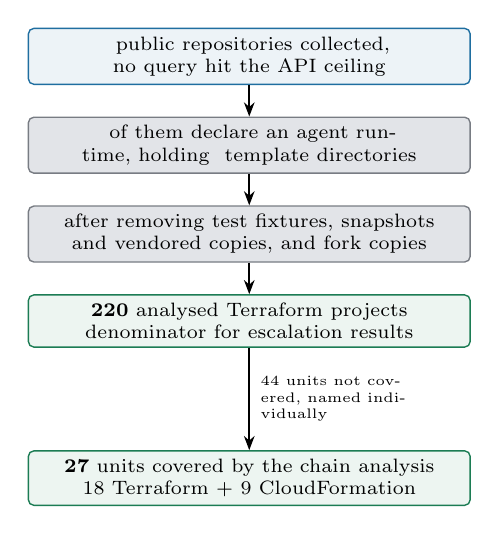
\begin{tikzpicture}[
  font=\scriptsize,
  box/.style={draw, rounded corners=2pt, align=center, inner sep=3pt,
              text width=54mm, minimum height=6mm, line width=0.5pt},
  keep/.style={box, draw=cIdentity, fill=cIdentity!8},
  narrow/.style={box, draw=cNeutral, fill=cFaint},
  final/.style={box, draw=cAccent, fill=cAccent!8},
  down/.style={-{Stealth[length=1.8mm]}, line width=0.6pt},
  side/.style={font=\tiny, align=left, text width=20mm, inner sep=1pt},
]

\node[keep] (a) {\textbf{\nReposCollected} public repositories collected, no
  query hit the API ceiling};
\node[narrow, below=4mm of a] (b) {\textbf{\nReposWithRuntime} of them declare
  an agent runtime, holding \textbf{\nTemplateDirs} template directories};
\node[narrow, below=4mm of b] (c) {after removing \nTemplateExcluded test
  fixtures, snapshots and vendored copies, and \nTemplateForkCopies fork
  copies};
\node[final, below=4mm of c] (d) {\textbf{\nProjects} analysed Terraform
  projects\\\scriptsize denominator for escalation results};
\node[final, below=13mm of d] (e) {\textbf{\nChainDenominator} units covered by
  the chain analysis\\\scriptsize \nChainTerraform Terraform $+$ \nChainCfn
  CloudFormation};

\draw[down] (a) -- (b);
\draw[down] (b) -- (c);
\draw[down] (c) -- (d);
\draw[down] (d) -- node[side, right=1mm]
  {\nChainNotCovered units not covered, named individually} (e);

\end{tikzpicture}
\caption{How the collection narrows to each denominator. The two shaded boxes
are different populations and the paper does not mix them: a rate over
\nProjects and a rate over \nChainDenominator answer different questions.}
\label{fig:pipeline}
\end{figure}


\subsection{Verification}

Numbers come from artifacts, the artifacts are rebuilt by one script, and a
verification pass re-derives every published figure from them.
Appendix~\ref{sec:repro} gives the commands. Where a second pass re-derived a
number from the raw source, Appendix~\ref{sec:claims} reports its precision;
where none did, it says so.

\section{Results}
\label{sec:results}

\subsection{Complete escalations}

Over the \nChainDenominator units the chain analysis covered, it found
\nChainsFound complete cross-agent escalations. With no event observed in
\nChainDenominator trials, the one sided 95\% upper bound on the rate is
\chainBound\%. The measurement is consistent with a true rate anywhere from
zero to about one deployment in ten.

The predicate does fire inside the wider set of \nProjects analysed projects.
\nEscalating configurations contain an escalation, \nEscalatingOwnResource of
them reaching a resource the same configuration itself writes, and
\nSurvivingTakeover of them retaining a takeover edge.

\nEscalatingSingleAgent of those \nEscalating configurations declare a single
agent, and the escalating principals are a continuous integration
deploy role, a service user, and a role that executes actions. They are single-identity
escalations, produced by the same predicate.

\subsection{Candidates blocked on one permission}

\nBlocked takeover candidates across \nBlockedConfigs configurations are
blocked, and every one of them is blocked by the same permission,
\iam{iam:PassRole}. This is the structural claim of
Section~\ref{sec:background} appearing in the measurement: there is no second
way around the pass.

The \nBlocked are not interchangeable. Figure~\ref{fig:blocked} sorts them by
what the principal and the target are, recovered from the raw Terraform rather
than from the analysis output. \nBlockedAgentToAgent are one agent reaching
another agent of the same deployment, which is the case this paper is about.
\nBlockedSingleAgent are in configurations that declare one agent, so the
precondition is present and the second agent is not. \nBlockedPrincipalNotAgent
have a principal that is not an agent execution role, such as a build role, and
\nBlockedTargetNotAgent have a target that is not one.

\begin{figure}[t]
\centering
\resizebox{\columnwidth}{!}{%
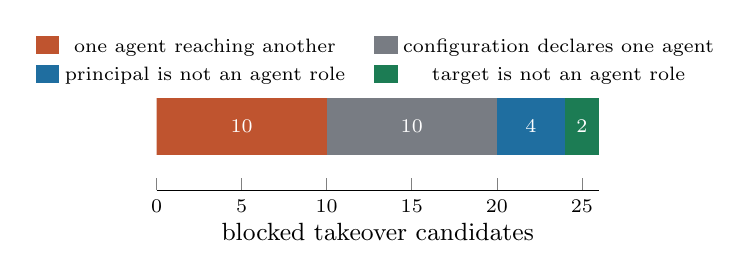
\begin{tikzpicture}
\begin{axis}[
  width=72mm,
  height=32mm,
  xbar stacked,
  xmin=0, xmax=26,
  bar width=7mm,
  axis y line=none,
  axis x line*=bottom,
  xtick={0,5,10,15,20,25},
  xlabel={\small blocked takeover candidates},
  xlabel style={font=\small, yshift=1mm},
  tick label style={font=\scriptsize},
  legend style={
    font=\scriptsize, draw=none, fill=none,
    at={(0.5,1.28)}, anchor=north, legend columns=2,
    /tikz/every even column/.append style={column sep=3mm}},
  nodes near coords={\scriptsize\pgfmathprintnumber\pgfplotspointmeta},
  every node near coord/.append style={text=white, anchor=center},
]
\addplot+[fill=cStored, draw=cStored] coordinates {(10,0)};
\addlegendentry{one agent reaching another}
\addplot+[fill=cNeutral, draw=cNeutral] coordinates {(10,0)};
\addlegendentry{configuration declares one agent}
\addplot+[fill=cIdentity, draw=cIdentity] coordinates {(4,0)};
\addlegendentry{principal is not an agent role}
\addplot+[fill=cAccent, draw=cAccent] coordinates {(2,0)};
\addlegendentry{target is not an agent role}
\end{axis}
\end{tikzpicture}}
\caption{The \nBlocked candidates blocked on \iam{iam:\allowbreak PassRole}, sorted by what
the principal and the target are. Only the first group,
\nBlockedAgentToAgent of \nBlocked, is one agent reaching another agent of the
same deployment. Each candidate was re-derived from the raw Terraform rather
than taken from the analysis output.}
\label{fig:blocked}
\end{figure}


Separately, \nPassRoleWide configuration grants \iam{iam:PassRole} broadly
enough to cover a role an agent in that same configuration runs as. That is the
one deployment in the corpus where the gate that blocks the other
\nBlocked candidates is already open.

\subsection{What an existing scanner reports on the same corpus}
\label{sec:baseline}

The property here is a relation between two resources, and rule based
scanners work on one. We ran Checkov, a widely used open source scanner for
infrastructure as code, over the same \nProjects configurations, on Terraform
with no network access and nothing else changed.

Checkov reports \nCheckovFailed findings from \nCheckovRules distinct rules,
and \nCheckovOnAgentRuntime of them take an agent runtime as their subject:
the resource type is not in its rule set, so these agents are invisible to it.
Its rules that span resources fired \nCheckovGraphFailed times.
\nCheckovRelationRules of the rule names that fired suggest a relation
between resources, and they concern cross-account access, cross-region
replication and load balancing, not two agents.

Most of those findings are about encryption and logging, which this paper
does not look at. A deployment can pass every rule in a mature rule set while
\nSharedRoleRuntimes of \nMultiAgentRuntimes multi-agent deployments run every
agent under one role.

\subsection{Agents sharing one execution role}

\begin{table}[t]
\centering
\caption{Multi-agent deployments and role sharing, counted two ways. A runtime
block carrying \texttt{count} or \texttt{for\_each} deploys more than one
agent, so the two columns answer different questions. The paper uses the
runtime column, and the artifact names the deployments that move.}
\label{tab:sharing}
\small
\setlength{\tabcolsep}{4pt}
\begin{tabular}{@{}lcc@{}}
\toprule
 & \textbf{by block} & \textbf{by runtime} \\
\midrule
Two or more agents               & \nMultiAgentBlocks & \nMultiAgentRuntimes \\
Of those, all on one role        & \nSharedRoleBlocks & \nSharedRoleRuntimes \\
\bottomrule
\end{tabular}
\end{table}

Table~\ref{tab:sharing} gives the role sharing census. \nSharedRoleRuntimes of
\nMultiAgentRuntimes multi-agent deployments run every agent under a single
execution role.

This is the finding with the most practical weight in the paper, and it is not
an escalation. Where the role is shared the attacker does not need the takeover
at all: the agents already hold identical permissions, so compromising any one
of them yields what all of them can reach. It also removes the account's
ability to attribute a call to an agent, because every call arrives under the
same role.

\subsection{CloudFormation}

The CloudFormation side of the collection holds \nCfnMultiRuntime templates
that declare more than one runtime. \nCfnAnalysed were analysed and contain
\nChainsFound chains. \nCfnUndecidable are undecidable: an intrinsic in a role
or runtime argument did not resolve, and the template is reported as such
rather than as clean.

\subsection{CDK}

The source scan flags \nCdkMultiRuntimeDirs CDK directories with more than one
runtime, \nCdkInScope after the exclusion rule of
Section~\ref{sec:methodology}. Reading a CDK role's policies out of the source
is a heuristic, so we synthesised instead.

Of the \nCdkInScope, \nCdkAnalysed synthesised and went through the exact
CloudFormation pipeline, recovering \nCdkRuntimes agent runtimes and
\nCdkEscalating escalations. Table~\ref{tab:cdk} gives the reasons the rest did
not synthesise. A failure to install a dependency and a failure to find an
application are different facts about the corpus.

\begin{table}[t]
\centering
\caption{Why \nCdkInScope CDK directories did or did not reach the analysis.
A directory that does not synthesise is not counted as clean.}
\label{tab:cdk}
\small
\begin{tabular}{lr}
\toprule
\textbf{Outcome} & \textbf{Directories} \\
\midrule
Synthesised and analysed                     & \nCdkAnalysed \\
\midrule
Synthesis failed                             & \nCdkFailSynth \\
Not a supported application layout           & \nCdkFailLanguage \\
Dependency install failed                    & \nCdkFailInstall \\
No \texttt{cdk.json} above the directory     & \nCdkFailLocate \\
\bottomrule
\end{tabular}
\end{table}

\subsection{What the CDK results add to the denominator}

\nCdkAnalysed directories is not \nCdkAnalysed applications.
\nCdkSampleCopies of them are the same AWS sample application carried into
\nCdkSampleCopies different repositories, at the same path inside each. By the
deduplication rule of Section~\ref{sec:methodology} those count once, which
leaves \nCdkDistinctApps distinct applications.

Adding them to the chain denominator gives \nChainDenominatorExt units with
\nChainsFound chains, and the one sided 95\% upper bound tightens from
\chainBound\% to \chainBoundExt\%. The first bound covers the deployments read
directly; the second adds the synthesised CDK applications.

\section{The Takeover in a Live Account}
\label{sec:case-study}

The corpus says the path is not completed in public infrastructure as code.
It does not say the path works. We built it in an AWS account to show that it
does, and to find out what actually gates it.

\subsection{Setup}

The account holds three agent runtimes and three execution roles. Two of the
roles differ in their policies. The third, \texttt{execC}, is identical to the
second in every way except its name.

The attacker is a separate principal whose only permission is the AWS managed
policy \iam{BedrockAgentCoreFullAccess}. It is given nothing else. In
particular it is given no direct access to the resource it will end up
reading.

A canary object sits in a bucket that only the victim's execution role can
read. A pre-check confirms the attacker cannot read it.

\subsection{Verdict rules}

Three rules are encoded in the harness. A verdict comes from reading the
runtime back from the platform and asking what role it says the runtime now
runs as, never from the request that was sent. An \texttt{AccessDenied} counts
as a block only when the message names \iam{iam:PassRole}; any other denial is
recorded as inconclusive, because a denial for an unrelated reason would
otherwise look like the control working. And role assumption is retried for
120 seconds, so a propagation delay is not recorded as a control.

\begin{figure}[t]
\centering
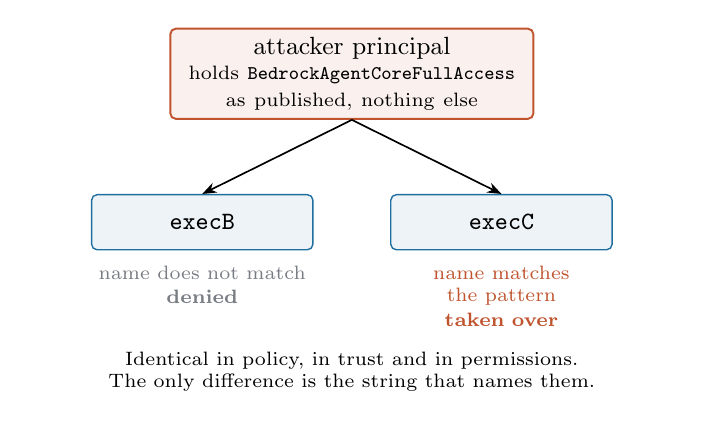
\begin{tikzpicture}[
  font=\small,
  atk/.style={draw, rounded corners=2pt, align=center, inner sep=3pt,
              text width=44mm, draw=cStored, fill=cStored!8, line width=0.7pt},
  same/.style={draw, rounded corners=2pt, align=center, inner sep=3pt,
               text width=26mm, minimum height=7mm, line width=0.5pt,
               draw=cIdentity, fill=cIdentity!8},
  verdict/.style={font=\scriptsize, align=center, inner sep=1pt,
                  text width=32mm},
  flow/.style={-{Stealth[length=1.8mm]}, line width=0.6pt},
]

\node[atk] (atk)
  {attacker principal\\[1pt]
   \scriptsize holds \iam{BedrockAgentCoreFullAccess}\\[-1pt]
   \scriptsize as published, nothing else};

% placed by explicit offset from the centre: anchoring to the box corners
% spreads them wider than the column
\node[same] (b) at ([shift={(-19mm,-13mm)}]atk.south) {\texttt{execB}};
\node[same] (c) at ([shift={( 19mm,-13mm)}]atk.south) {\texttt{execC}};

\draw[flow] (atk.south) -- (b.north);
\draw[flow] (atk.south) -- (c.north);

\node[verdict, below=1.5mm of b, text=cNeutral]
  {name does not match\\[1pt]\textbf{denied}};
\node[verdict, below=1.5mm of c, text=cStored]
  {name matches the pattern\\[1pt]\textbf{taken over}};

\node[font=\scriptsize, align=center, text width=80mm]
  at ([shift={(0mm,-32mm)}]atk.south)
  {Identical in policy, in trust and in permissions.\\
   The only difference is the string that names them.};

\end{tikzpicture}
\caption{The control. Two victim roles are built identically and differ only
in name. The attacker holds one AWS managed policy, attached as published,
with no inline statement added. One role is taken over and the other is
refused, so what separates one agent from another agent's role is a check on
the kind of role rather than on whose role it is, and the account's own
default role names satisfy that check.}
\label{fig:control}
\end{figure}


\subsection{The cells}

The experiment is nine cells, each a question with an outcome recorded to a
file at the time it ran. Table~\ref{tab:cells} lists them. The design is a
control and a treatment that differ by exactly one permission, plus the cells
that close off the ways the result could be an artefact.

\begin{table}[t]
\centering
\caption{The nine cells of the live experiment and the verdict each
recorded. The attacker holds the managed policy in every cell except the
first. Control and treatment differ by one inline grant and nothing else.}
\label{tab:cells}
\small
\begin{tabular}{p{18mm}p{39mm}p{15mm}}
\toprule
\textbf{Cell} & \textbf{Question} & \textbf{Verdict} \\
\midrule
positive control & can the operator replace the runtime's artifact at all &
  allowed \\
control & can the attacker, holding only the managed policy, replace a
  sibling's artifact & denied \\
treatment & the same, with one inline \iam{iam:\allowbreak PassRole} grant
  on the target role added & allowed \\
recheck & the same again with that grant removed & denied \\
\midrule
name condition & the same as the control, changing only the victim role's
  \emph{name} to match \iam{*Bedrock\allowbreak AgentCore*} & allowed \\
\midrule
gain & does the target role reach something the attacker does not & gain \\
effect & does the replaced code run and return the canary & canary
  returned \\
falsification & give the attacker directly what the target holds, then take
  over anyway & allowed, no gain \\
\midrule
persistence & after the attacker loses every permission, does the operator's
  own call still reach the planted code & persists \\
\bottomrule
\end{tabular}
\end{table}

The control and the recheck both end in an implicit deny, and the policy
simulator reports no matching statement. The treatment differs from them by a
single inline grant, and the recheck removes that grant and recovers the deny,
so the allow is attributable to the grant rather than to a propagation delay
or to a change in the account between runs.

The falsification cell is the one that constrains the predicate rather than
the platform. The attacker is given, directly, the thing the target role
holds. The takeover still succeeds and the API exchange is identical to the
treatment's. Equation~\ref{eq:esc} does not fire, because the reach is already
inside $\auth$.

\subsection{Result}

The attacker replaced the sibling runtime's definition. The platform reported
the runtime as running under the victim's execution role. The replaced code
executed, read the canary, and returned it to the attacker, who could not read
it directly before or after.

The planted code carries no SDK, because the runtime image has none, so it
signs its own request with a short standard library implementation. It
reports the \emph{name} of its credential source and the \emph{names} of the
AWS environment variables it can see, never a value.

\subsection{What the gate turned out to be}

The most useful cell is the name condition, because it changes one thing. The
victim role in that cell is identical to the control's in its policies, its
trust policy and its permissions. Only its name differs, and it differs so as
to match \iam{*BedrockAgentCore*}, which is how the AWS console names the
execution roles it creates for this service.

With that single change, and with the attacker still holding only
\iam{BedrockAgentCoreFullAccess} and no inline grant at all, the takeover
succeeded. The control denied the same request against the same kind of role
under a different name.

So the control that stands between two agents in a default deployment is a
string match on a role name, not a statement about which agent owns which
role. An operator who follows the console's own defaults, and grants the
vendor's own managed policy, has the path open.

This is a result about the condition rather than about the policy being
permissive. A policy named for full access that passed any role without a
condition would carry no claim to separate anything, and there would be
nothing here to report. The \iam{iam:PassRole} statement in v21 is not
unscoped: it is narrowed twice, by a resource pattern over the role's name
and by a condition on the service the role may be passed to, and narrowing a
statement is a decision to restrict what the permission reaches. What the
experiment establishes is that the restriction chosen, a glob over the name, is
not a restriction on ownership, and that the service's own console produces
names on the inside of it. The same statement with the role's ARN in place of
the pattern refuses the cell that succeeded, which
Section~\ref{sec:arn-repair} measures rather than asserts.

\subsection{What the second permission buys}

The canary could also have been read through the command route, with one
permission and no \iam{iam:PassRole}. The ninth cell measures what the extra
permission buys. It runs after the name condition, so the attacker holds only
the managed policy, and it aims the planted code at the canary through the
environment variables of the same \api{Update\allowbreak AgentRuntime} call.
Then every policy on the attacker principal is detached. The attacker's next
update of that runtime is refused with an \texttt{AccessDenied} naming
\iam{bedrock-agentcore:\allowbreak Update\allowbreak AgentRuntime}, and the
simulator reports an implicit deny on the canary.

With the attacker in that state, the operator invokes the runtime through its
ordinary endpoint. The response carries the attacker's marker, names instance
metadata as its credential source, and contains the canary value.

A stolen credential stops working when the principal that took it is disabled.
A replaced artifact keeps answering the agent's own callers under the victim's
role, with no attacker principal involved, until someone compares the running
artifact against the one that was meant to be there. That comparison is the
detection in Section~\ref{sec:defences}.

\section{\foundry: Connections Instead of Declared Agents}
\label{sec:foundry}

The analysis reads agents out of a deployment, so it needs the deployment to
declare them. On \foundry it does not. We collected \nFoundryRepos
repositories, \nFoundryFiles files and \nFoundryDirs template directories, and
\nFoundryAgentDirs of those directories declare an agent as a deployed
resource. Agents there are created at run time through the service's own APIs,
so the deployment-time artifact the AWS analysis reads does not exist.

No rate comparable to the AWS one can be computed from these templates.

What \foundry templates do carry is \emph{connections}, and a connection's
\api{authType} decides whether a call presents a directory identity or a
credential stored in the connection. Where several agents share a project, a
stored credential is presented identically by all of them, so the target
cannot tell them apart and each agent reaches everything the connection is
trusted with. That is the same loss of separation the role sharing of
Section~\ref{sec:results} produces on AWS, reached by a different route.
Figure~\ref{fig:authtypes} gives the distribution:
\nAuthStoredCredential of \nFoundryAuthValues assigned values, about
\pctAuthStoredCredential percent, store a credential rather than presenting an
identity. \api{authType} is also a field on three unrelated Azure providers,
so the count is taken only inside directories declaring a connection resource.
No template sets an identity type scoped to an individual agent; those values
appear in parameter lists as allowed values only.

\begin{figure}[t]
\centering
\resizebox{\columnwidth}{!}{%
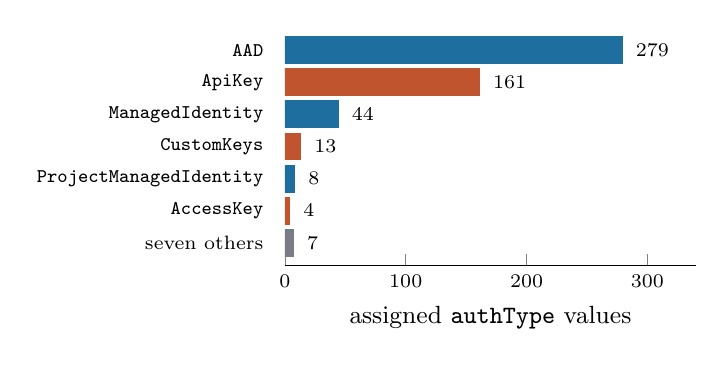
\begin{tikzpicture}
\begin{axis}[
  width=68mm,
  height=46mm,
  xbar,
  y dir=reverse,
  xmin=0, xmax=340,
  ymin=-0.7, ymax=6.7,
  bar width=3.4mm,
  /pgfplots/bar shift=0pt,
  axis x line*=bottom,
  axis y line*=left,
  y axis line style={draw=none},
  ytick={0,1,2,3,4,5,6},
  yticklabels={%
    \texttt{AAD},
    \texttt{ApiKey},
    \texttt{ManagedIdentity},
    \texttt{CustomKeys},
    \texttt{ProjectManagedIdentity},
    \texttt{AccessKey},
    seven others, one each},
  ytick style={draw=none},
  tick label style={font=\scriptsize},
  xtick={0,100,200,300},
  xlabel={\small assigned \texttt{authType} values},
  xlabel style={font=\small},
  nodes near coords={\scriptsize\pgfmathprintnumber\pgfplotspointmeta},
  every node near coord/.append style={anchor=west, xshift=0.5mm},
]
\addplot[xbar, bar shift=0pt, fill=cIdentity, draw=cIdentity] coordinates {(279,0)};
\addplot[xbar, bar shift=0pt, fill=cStored,   draw=cStored]   coordinates {(161,1)};
\addplot[xbar, bar shift=0pt, fill=cIdentity, draw=cIdentity] coordinates {(44,2)};
\addplot[xbar, bar shift=0pt, fill=cStored,   draw=cStored]   coordinates {(13,3)};
\addplot[xbar, bar shift=0pt, fill=cIdentity, draw=cIdentity] coordinates {(8,4)};
\addplot[xbar, bar shift=0pt, fill=cStored,   draw=cStored]   coordinates {(4,5)};
\addplot[xbar, bar shift=0pt, fill=cNeutral,  draw=cNeutral]  coordinates {(7,6)};
\end{axis}
\end{tikzpicture}}
\caption{\api{authType} across the \nFoundryAuthValues assigned values in the
\nFoundryAuthDirs directories that declare a connection resource. Blue
presents a directory identity, orange stores a credential in the connection.
The last row collects seven values that occur once each, which the artifact
names. \nAuthStoredCredential of \nFoundryAuthValues store a credential rather
than presenting an identity.}
\label{fig:authtypes}
\end{figure}


\section{External Validation}
\label{sec:validation}

\paragraph{A check contributed to an open source scanner.}
The \foundry result of Section~\ref{sec:foundry} is expressible as a rule
about deployed state, so we implemented it as a check for Prowler, an open
source cloud security scanner, and opened it as pull request 13306 on
\texttt{prowler-cloud/prowler}. The check
reports connections whose \api{authType} presents a credential stored in the
connection rather than a directory identity, at both account and project
level, and reports a scope whose connections could not be listed as manual
rather than leaving it out.

The review that followed changed the code. An automated reviewer found that a
project whose connections could not be listed was dropped from the results
instead of reported, which is the same class of error the check was written to
avoid, one level down. It also found that a finding carried no region, because
a connection has no location of its own and the parent account's was not being
used. Both are fixed, with tests, and the fix for the first was extended to the
account's own scope, where the same gap existed and the review had not looked.

The pull request is open and under review on 8 November 2026, with the two
review findings fixed and no maintainer decision yet.

\paragraph{A report to a vendor sample repository.}
A separate finding concerns a \foundry starter template whose connection
module defaults \api{isSharedToAll} to true, and whose \nFoundryTemplateShared
call sites all set it to true. Where a project holds more than one agent,
every connection is reachable by all of them, and the
\nFoundryTemplateApiKey that carry an \api{ApiKey} present a stored
credential the target cannot attribute to an agent. The
module is byte identical in \nFoundryTemplateCopies copies across
\nFoundryTemplateRepos repositories, so it is filed once against the
template repository rather than in each of them. It is issue 73 on
\texttt{Azure-Samples/\allowbreak azd-ai-starter-basic}, open at the time of
writing.

\paragraph{Disclosures to deployment owners.}
The deployments behind the findings in Section~\ref{sec:results} are public
repositories with identifiable owners. We sent \nDisclosureReports reports on 8 November 2026,
covering \nDisclosureRepos repositories: \nDisclosureIssues
as public issues on repositories whose published policy allows one, and
\nDisclosureEmails to a vendor security address, for the organisation whose
policy asks that no public issue be opened. Each report names the shared
execution role, the file and line it is declared on, and the change that
removes it.

No reply had arrived by 8 November 2026. Each report asked whether the owner
would agree to be named here, so the repositories are not identified.

\section{Defences and Detection}
\label{sec:defences}

\subsection{What an operator can do}

\paragraph{Give each agent its own execution role.}
This is the one with the largest effect and the clearest evidence behind it:
\nSharedRoleRuntimes of \nMultiAgentRuntimes multi-agent deployments do not do
it today. A shared role makes the takeover unnecessary, because the agents
already hold the same permissions, and it removes the account's ability to
say which agent made a call. Separating the roles does not by itself stop the
takeover, but it is what makes every other control in this list possible.

\paragraph{Name the role instead of matching its name.}
The gate in the vendor's managed policy is a resource pattern over the role
name, so two agents whose roles both match \iam{*BedrockAgentCore*} are not
separated by it at all. A per agent policy granting \iam{iam:PassRole} on the
exact role ARN the agent needs, in place of
\iam{BedrockAgentCoreFullAccess}, names the role instead of matching a
pattern.

This is worth stating as a defence because the vendor's own policy checker
does not treat the pattern as a problem. IAM Access Analyzer raises
\texttt{PASS\_ROLE\_WITH\_STAR\_IN\_RESOURCE} on \iam{iam:PassRole} with a
wildcard resource, and its reference documentation records an exception for
this exact shape: a resource such as \iam{arn:aws:iam::*:role/Service*} may
produce no finding, because some services put their own namespace in the names
of the roles they create~\cite{awsAccessAnalyzerChecks}. The convention that
makes the pattern look specific is the same convention that places every
agent's execution role inside it, so an operator running the vendor's checker
over the vendor's policy is told nothing.

\paragraph{Narrow the trust policy.}
The documented trust policy for an execution role scopes
\iam{sts:AssumeRole} with \iam{aws:SourceArn} set to a wildcard over the whole
account. Replacing the wildcard with the specific runtime ARN closes the
target side of the edge, and the role then cannot be reused by
another runtime.

\paragraph{Separate the identity that deploys from the identity that runs.}
\api{UpdateAgentRuntime} is a deployment operation. An agent's own execution
role rarely needs it, and where it does the grant should name the runtime it
may update. The corpus contains \nBlockedAgentToAgent candidates that are one
agent reaching another and are held back only by \iam{iam:PassRole}; in those
deployments the update permission is already present on the wrong identity.

\paragraph{Constrain the command route as well.}
The controls above govern who may replace an agent's artifact. They do nothing
about the permission that runs a command inside an existing runtime, which
reaches the same role more cheaply and has a service control policy of its
own~\cite{garcia2026agentcorepaths}. Apply both.

\subsection{Whether the first defence refuses the cell that succeeded}
\label{sec:arn-repair}

The defence above is a proposal until something evaluates it, so it is
evaluated here with the engine that decides the real call. The
\iam{iam:PassRole} statement is read from the live managed policy rather than
retyped, a second copy is made with only the \iam{Resource} element replaced
by the ARN of the one role an agent is entitled to pass, and both are put to
\api{SimulateCustomPolicy} against three targets with
\iam{iam:PassedToService} set to the service. Nothing is created and no
runtime is involved; the artifact is
\texttt{evaluation/\allowbreak benchmark/\allowbreak arn\_condition\_repair.json}
and the script that writes it reads the policy afresh on each run.

Table~\ref{tab:repair} gives the \nRepairDecisions decisions. The row that
matters is the second: the shipped statement is \repairShippedSibling{} to
pass a sibling agent's role, because the console named that role inside the
pattern, and the same statement pinned to an ARN is \repairPinnedSibling. The
last row is the one that makes it a repair and not a removal, since the
pinned statement still allows the agent to pass its own role, which is what
the permission is for.

\begin{table}[t]
\centering
\caption{The first defence, put to the IAM policy simulator. The shipped
statement and the same statement with its resource pinned to one role ARN,
each against three targets. The repair denies the cell that succeeded in
Section~\ref{sec:case-study} and leaves the agent's own pass working.}
\label{tab:repair}
\small
\begin{tabular}{@{}llL{22mm}@{}}
\toprule
\textbf{Role being passed} & \textbf{Shipped v21} & \textbf{Pinned to one ARN} \\
\midrule
the agent's own role & allowed & allowed \\
a sibling the console named & allowed & denied \\
a sibling named anything else & denied & denied \\
\bottomrule
\end{tabular}
\end{table}

Two limits belong with this. The simulator decides authorisation, so what is
measured is the decision and not the \api{UpdateAgentRuntime} call being
refused end to end; the live cells in Section~\ref{sec:case-study} are what
show the call itself. And the repair moves the problem rather than dissolving
it: an account now has to get one policy right per agent, where before it
attached one policy everywhere, which is work that falls on whoever writes the
deployment.

\subsection{What an operator cannot fix this way}

Scoping an agent's data permissions does not help: agent~A never touches
agent~B's data, because the code it installs runs as agent~B and uses
agent~B's own permissions. A deployment where every role is perfectly scoped to its own agent is still
exposed to it. Controls at the model
layer do not help either, because the cloud permissions downstream are the
same whatever ran the attacker's code.

\subsection{What the analysis hands an operator}

A rule based scanner returns a verdict: the deployment violates the rule or it
does not. On this corpus that verdict is uninformative, because the resource
type is not in the rule set and all \nCheckovFailed findings are about
something else. But the deeper limitation is the shape of the answer rather
than the coverage. A deployment that is one grant away from a cross-agent
takeover and a deployment that is nowhere near one both come back clean, and
nothing in the output separates them.

Evaluating each delegation rule as a conjunction changes the shape of the
answer. When a rule does not fire, the analysis knows which conjunct failed,
so the output is not ``no path'' but ``no path, and this is the term that is
missing''. Over this corpus that term is the same one every time: all
\nBlocked candidates lack \iam{iam:PassRole} on the target role, and
Algorithm~\ref{alg:reach} carries the witness, so each one names the file and
the principal a reader can open.

Three things follow for an operator, and they are properties of the output
format, not new measurements. A blocked candidate is a ranking, because
a deployment one permission from a takeover is a different risk from one that
is several. It is also a specific instruction, since the permission not to
grant is named rather than inferred. And it is a regression test: the
\nPassRoleWide configuration where that permission is already granted broadly
is the same finding with the distance at zero, which is how a deployment
crosses from one class to the other when somebody widens a policy. The
numbers in Section~\ref{sec:results} are a census of the corpus; the same
output on one deployment is a work list.

\subsection{Detection}

Two signals follow directly from the mechanism, and both are available in
ordinary cloud audit logs.

The first is an \api{UpdateAgentRuntime} call whose \api{roleArn} differs from
the runtime's previous value. A deployment pipeline changes the artifact often
and the role almost never, so a change of role on an existing runtime is rare
enough to alert on rather than to sample.

The second is an \api{UpdateAgentRuntime} call made by a principal that is
itself an agent execution role. Agents are not usually deployers. Neither
signal is specific to an attack; both are specific enough to review.

Both miss the name condition cell of Section~\ref{sec:case-study}, where the
role does not change and the attacker is an ordinary principal. The third
signal is a comparison, not an event: reading each runtime's artifact
back and checking it against the object the pipeline published names the
runtimes whose code is no longer what was deployed. It is the only one of the
three that still fires once the attacker is gone.

\subsection{What the platform could change}

If replacing an artifact and changing an execution role were separate
operations with separate permissions, the takeover path would need two grants
instead of one, and the common case of updating an agent that keeps its
identity would stop requiring \iam{iam:PassRole} at all. Short of that, a
condition key expressing ownership instead of a name pattern would let the
managed policy say what it appears to say.

\section{Limitations}
\label{sec:limitations}

\paragraph{The corpus is small.}
Everything measured is code published on a public host, so private deployments and those built by hand in a console cannot
appear, and we cannot estimate how the populations differ.

\paragraph{The second passes share the first's blind spots.}
Each precision in Appendix~\ref{sec:claims} comes from a pass that re-derived
that number from the raw source with its own patterns. A separate pass
re-derives three of the published figures with deliberately different
patterns, and agrees with all three. The two disagreements it produced
earlier were resolved against it: one had matched a wildcard in a
neighbouring policy statement, the other a resource type from a different
Azure provider. Neither kind of pass can catch an error in the collection,
because both use the same collection.

\paragraph{Most claims have no precision at all.}
\nClaimsWithPrecision of \nClaims claims in this paper have a measured
precision. The rest are reported as counts with their population, and
Appendix~\ref{sec:claims} marks each one.

\paragraph{Undecidable templates.}
\nCfnUndecidable CloudFormation templates, and the Terraform expressions
reported per project in the artifact, do not resolve to a value the analysis
can use. They are reported
as undecidable rather than as clean.

\paragraph{The live demonstration is one account.}
Section~\ref{sec:case-study} shows the mechanism works with vendor default
role names and a vendor managed policy. One account is enough to show a
mechanism exists and not enough to say anything about how often that
configuration occurs.

\section{Related Work}
\label{sec:related}

\subsection{Reasoning about cloud access control}

Zelkova encodes AWS policies into SMT and answers questions about them
exactly, such as whether one policy is more permissive than
another~\cite{backes2018zelkova}. What it answers is a question about a policy
or a pair of policies. The property here belongs to a deployment: it needs the
principals, the agent runtimes, and the arguments that bind one to another.
Asking whether role A's policy is more permissive than role B's does not
reveal that A can replace what B runs.

\subsection{Multi-step attacks and escalation paths}

Shevrin and Margalit use model checking to find multi-step IAM attacks, where
each step is an API call that changes what the attacker can do
next~\cite{shevrin2023multistep}. TAC combines static and dynamic information
to detect IAM privilege escalation~\cite{hu2023tac}. Both treat escalation as
a path rather than a single bad grant, which is the stance here.

The difference is what sits at the end of an edge. There the attacker moves
between IAM principals: it assumes a role, creates a key, attaches a policy.
Those edges exist here too. The edge this paper adds does not move between
principals at all: the attacker rewrites the \emph{workload} an existing
principal runs, and nothing about that principal changes. An analysis built on
principal to principal transitions has no place to put that edge.

A second difference is the input: model checking needs a deployed account,
while \tool runs against the source, which is what makes the measurement in
Section~\ref{sec:results} possible and puts a finding in review.

\subsection{Reporting on this platform}
\label{sec:industry}

Cross-agent escalation on \agentcore is not an unreported problem, and the
term is not ours. Unit~42 disclosed that the execution role the AgentCore
starter toolkit creates carries wildcard scopes, so a compromised agent can
read other agents' memory, pull their container images, and invoke
them~\cite{hadad2026godmode}. Mitigant built four paths on that same role,
including a cross-agent runtime hijack~\cite{torkura2026agentsore}. Rehberger describes cross-agent escalation
in a different setting, where one agent approves actions for
another~\cite{rehberger2025freeeachother}.

BeyondTrust is the closest: \iam{bedrock-agentcore:\allowbreak Invoke\allowbreak AgentRuntimeCommand}, on
its own, runs a
command as root inside an existing runtime's sandbox, and the platform's
metadata service returns that runtime's execution role
credentials~\cite{garcia2026agentcorepaths}. One permission, no
\iam{iam:PassRole}, no change to the deployment. Its \iam{iam:PassRole} chains
are create variants, for when no runtime carries the role the attacker wants.

\paragraph{Two routes, and the one this paper takes.}
The two answer different questions. Theirs reads a credential and leaves the
agent as it was; a rotation ends it, and the command lands in the log group
the platform creates for the runtime. Replacing the artifact leaves the agent
answering its own callers with attacker code until someone compares the
deployed artifact against what was meant to be there. Section~\ref{sec:case-study}
measures that difference: with every policy detached from the attacker
principal, the operator's own call to the runtime still returns the planted
code's answer, carrying the victim role's data. The cost of that durability is
a second permission, always \iam{iam:PassRole}.
\api{UpdateAgentRuntime} appears in none of the reporting above.

\paragraph{The gate is a name match.}
The wildcard execution role of the earlier reports is a misconfiguration, and
the fix is to scope it. Section~\ref{sec:case-study} isolates a different
control: with the attacker holding only \iam{BedrockAgentCoreFullAccess}, the
single variable that decides the outcome is whether the victim role's
\emph{name} matches \iam{*BedrockAgentCore*}, which the console's own default
names do. BeyondTrust names that managed policy as over broad and proposes a
service control policy keyed on \iam{aws:PrincipalArn}; the role name
condition inside the policy is not examined.

\paragraph{Prevalence.}
Each of those reports is a single scenario in a controlled account. None
measures how often the preconditions occur, and none reads a deployment before
it exists.

\subsection{Infrastructure as code}

Rahman et al.\ catalogue recurring security smells in IaC scripts and show
they are common in public repositories~\cite{rahman2019sevensins}, and open
scanners implement rule sets of that kind. The unit of analysis differs: a
smell fires on one resource, while the property here is a relation between two
resources in the same file. A deployment where every resource passes every
rule is the deployment this paper is about.

\subsection{Security of LLM agents}

Abdelnabi et al.\ show that content an LLM-integrated application retrieves
can carry instructions the application then
follows~\cite{abdelnabi2023notwhat}, which is why
Section~\ref{sec:threat-model} starts from attacker code running as one
agent. That literature stops at the boundary of the agent's own capabilities;
this paper starts there and asks what the account looks like when the agent is
one of several.

\section{Conclusion}
\label{sec:conclusion}

Managed agent platforms put several identities in one account. The question
that matters is not what one agent can reach, but what it can reach by going
through another agent, and that does not fit a single identity analysis. We
stated it as a set difference, implemented it, and ran it over public AWS
deployments. The corpus contains \nChainsFound complete
cross-agent escalations, which supports an upper bound of \chainBound\% and
nothing stronger.

Two results sit beside that zero. Replacing
what an agent runs cannot avoid \iam{iam:PassRole}, because one API call
decides the code and the identity together, and in a live account an attacker
holding the vendor's own managed policy completed that path against a role the
vendor's own console had named. And in the deployments where more than one
agent exists, \nSharedRoleRuntimes of \nMultiAgentRuntimes already run every
agent under one role, which makes the escalation unnecessary and makes the
account unable to tell its agents apart.

The defence follows from that: give each agent its own execution role, and
treat \iam{iam:PassRole} over an agent's execution role as a grant of that
agent's permissions to whoever holds it.


\section{Availability}
\label{sec:availability}
\tool, the analysis, the harness that produced every artifact, and the lab
that builds and tears down the live demonstration are available at
\url{https://github.com/sarahda/agent-pathtriage}.

Every number in this paper is defined once in \texttt{numbers.tex}, and each
definition names the artifact it was read from. One command rebuilds the
artifacts, and a verification pass re-derives the published figures from them,
so a reader can check that the paper and the evidence agree without rerunning
the collection. The live demonstration creates and deletes its own AWS
resources and reports the names of credential sources rather than their
values.


\bibliographystyle{ACM-Reference-Format}
\bibliography{refs}

\appendix
\section{Claims and Second Checks}
\label{sec:claims}

Table~\ref{tab:claims} lists the claims that carry a population and a second
check. A blank means no second check.

The last column names its metric in every row, because the table holds two.
\emph{Precision} is the share of reported items a second pass, reading the raw
source, agreed with. \emph{Recall} is the share of known planted paths the
analysis recovered, measured against IAM-Vulnerable. They are not comparable.
The table comes from
\texttt{evaluation/\allowbreak benchmark/\allowbreak claim\_precision.json}.

\begin{table}[t]
\centering
\caption{The \nClaims claims, with the \nClaimsWithPrecision that carry a
measured precision and the two that carry a recall. Each value names its own
metric, because the two are not the same kind of number.}
\label{tab:claims}
\scriptsize
\setlength{\tabcolsep}{3pt}
\begin{tabular}{@{}p{30mm}p{15mm}p{20mm}p{13mm}@{}}
\toprule
\textbf{Claim} & \textbf{Number} & \textbf{Population} & \textbf{Second check} \\
\midrule
\multicolumn{4}{@{}l}{\emph{Recovery of known paths (IAM-Vulnerable)}} \\
\midrule
Delegation paths recovered once hand-offs are followed & \recallDelegation recall & IAM-Vulnerable delegation paths & \\
The same paths seen by a check that looks at one identity at a time & \recallSingleIdentity recall & IAM-Vulnerable delegation paths & \\
\midrule
\multicolumn{4}{@{}l}{\emph{Counts over the corpus}} \\
\midrule
Templates declaring two or more agents & \nMultiAgentBlocks & \nProjects analysed projects & \precMultiAgent precision \\
Templates running every agent under one execution role & \nSharedRoleBlocks of \nMultiAgentBlocks & the \nMultiAgentBlocks multi-agent templates & \precSharedRole precision \\
Resource-scope gaps adjudicated by hand & \nScopeGapsFlagged flagged & every gap the pass produced, none sampled & \\
A flagged gap covers a resource another agent in the same template owns & \nScopeGapsCrossAgent of \nScopeGapsWithSecondAgent & the \nScopeGapsWithSecondAgent flagged gaps in templates with a second agent & hand adjudicated \\
Takeover candidates blocked only on \iam{iam:PassRole} & \nBlocked across \nBlockedConfigs projects & \nProjects analysed projects & \\
Blocked candidates that are one agent reaching another & \nBlockedAgentToAgent of \nBlocked & the \nBlocked blocked candidates & every candidate re-read \\
Cross-agent escalation found in the corpus & \nChainsFound of \nChainDenominator & units the chain analysis covered & \\
Projects granting \iam{iam:PassRole} over a role an agent runs as & \nPassRoleWide of \nProjects & \nProjects analysed projects & \\
CDK apps running several runtimes under one role & \nCdkSharedRoleApps & the CDK apps the source scan flagged & \precCdkSharedRole precision \\
Foundry template directories holding an agent declaration & \nFoundryAgentDirs of \nFoundryDirs & \nFoundryRepos repositories, \nFoundryFiles files & \\
Foundry connection \api{authType} values, by type & see Figure~\ref{fig:authtypes} & \nFoundryAuthValues assigned values & \\
Connections that pick an agent scoped auth type & \nFoundryAgentAuthValues of \nFoundryAuthValues & \nFoundryAuthValues assigned values & \\
\bottomrule
\end{tabular}
\end{table}

\section{Reproducing the Results}
\label{sec:repro}

Every number is produced by a script and stored under
\texttt{evaluation/benchmark/}. This appendix says how to rebuild them.

\subsection{Three layers, by cost}

\paragraph{One configuration, seconds.}
Point the tool at a directory of Terraform.

\begin{lstlisting}
pip install -e .
python3 -m agentpathtriage.cli --path <dir> --json out.json
\end{lstlisting}

The output carries, per principal, $\auth$, the difference
$\eff \setminus \auth$, and a witness path for each element of it.

\paragraph{The artifacts, without recollecting the corpus, minutes.}
One command rebuilds the artifacts from the stored corpus and checks each
published figure against the artifact it came from.

\begin{lstlisting}
python3 evaluation/reproduce.py          # fast tier
python3 evaluation/reproduce.py --full   # add corpus walks
python3 evaluation/reproduce.py --full --budget 120
\end{lstlisting}

The fast tier skips the passes that walk every template, and
\texttt{--budget} takes seconds and slices those walks. A run reports each
check as a pass or as a failure naming the figure and the artifact that
disagree.

\paragraph{Collecting the corpus again, hours.}
Re-running the collection produces a different corpus as repositories change,
so the stored corpus is the unit of reproducibility and the scripts repeat the
method rather than the corpus.

\subsection{What each artifact backs}

\begin{table}[h]
\centering
\scriptsize
\setlength{\tabcolsep}{3pt}
\caption{Artifact to result, for the figures this paper asserts.}
\label{tab:artifacts}
\begin{tabular}{@{}p{33mm}p{38mm}@{}}
\toprule
\textbf{Artifact} & \textbf{Backs} \\
\midrule
\texttt{corpus\_takeover\_census} & \nProjects projects, \nBlocked blocked,
  the \nEscalatingSingleAgent escalations \\
\texttt{blocked\_takeover\_\allowbreak source\_check} & the four way split of
  Figure~\ref{fig:blocked} \\
\texttt{shared\_role\_corrected} & Table~\ref{tab:sharing}, both columns \\
\texttt{chain\_cfn\_corpus} & \nChainDenominator units, \chainBound bound \\
\texttt{cdk\_synth\_chain} & Table~\ref{tab:cdk},
  \nCdkDistinctApps distinct apps \\
\texttt{foundry\_recon} & Figure~\ref{fig:authtypes}, the
  \nFoundryAuthValues values \\
\texttt{claim\_precision} & Table~\ref{tab:claims} \\
\bottomrule
\end{tabular}
\end{table}

\subsection{The live demonstration}

The experiment of Section~\ref{sec:case-study} creates real AWS resources.

\begin{lstlisting}
cd attacks/passrole_runtime_takeover
python3 lab.py setup        # 3 runtimes, 3 roles, 1 attacker
python3 exploit.py <cell>   # one of the first eight cells
python3 persistence.py      # the ninth, after name-condition
python3 lab.py teardown
python3 teardown_verify.py  # reads the account back
\end{lstlisting}

Every name carries a random suffix per run. Each cell writes its question, the
request, the verdict and the time to \texttt{runs/}, which is where
Table~\ref{tab:cells} comes from. \texttt{teardown\_verify.py} separates a
resource still deleting from one left behind.


\end{document}
